% !TEX root = sn1604_wifes.tex

\begin{figure*}[tb!]
   \centering
   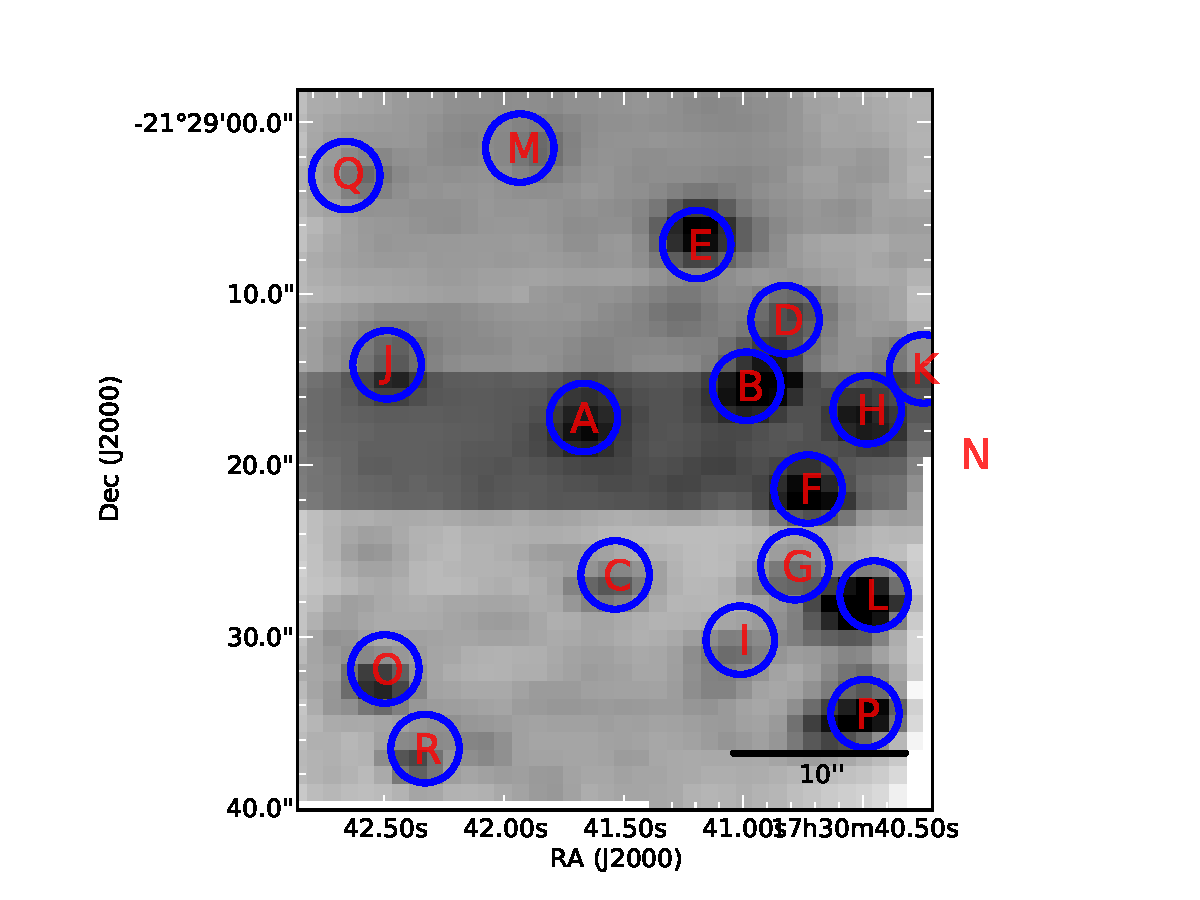
\includegraphics[width=.49\textwidth, bb = 0 0 500 400,clip]{\plotdir /sn1604_data_candidates.pdf} 
   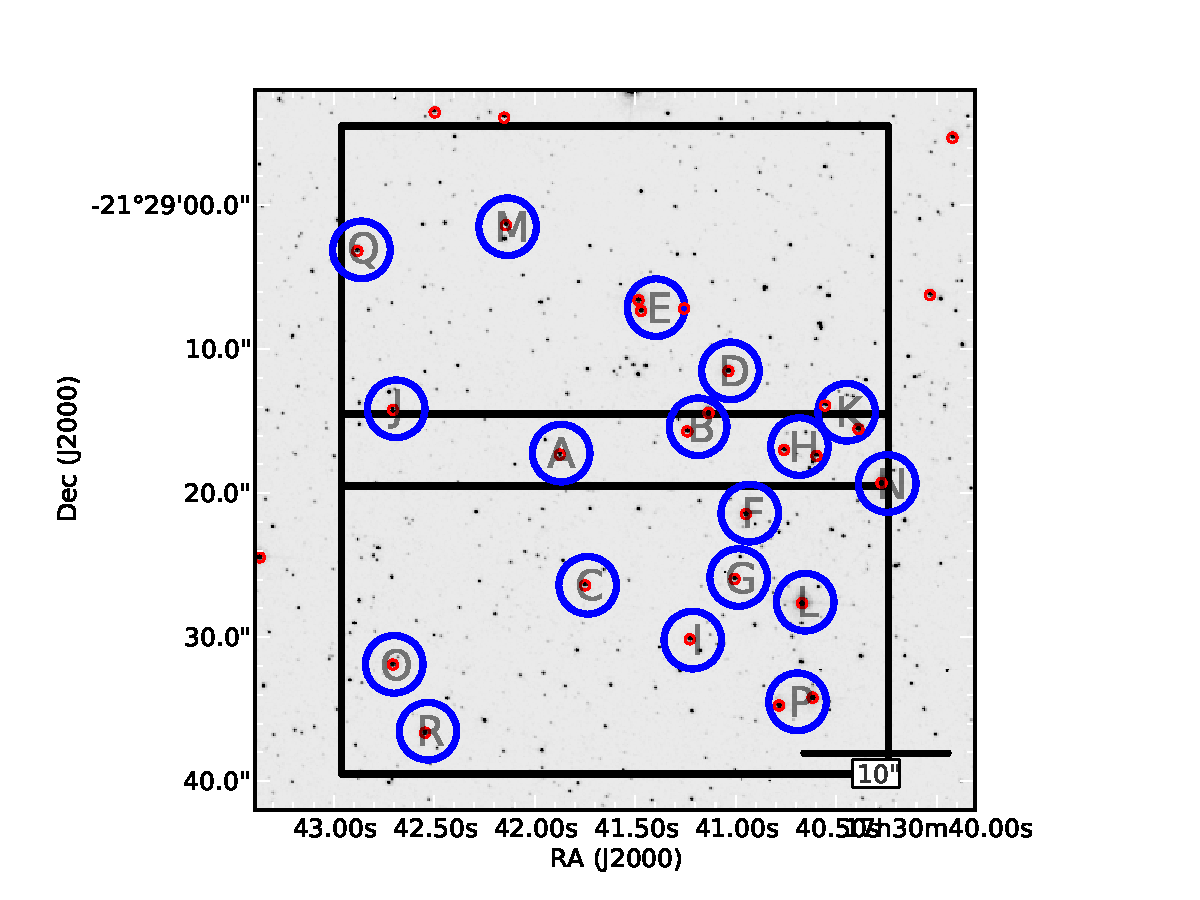
\includegraphics[width=.49\textwidth, bb = 0 0 500 400,clip]{\plotdir /sn1604_hst_candidates.pdf}
   \caption{\textbf{Left panel:} The combination of a median (in the spectral direction) of two of our spectral cubes. The extraction regions marked in blue. The seeing is comparable to the 2MASS, enabling a direct comparison of 2MASS magnitudes and the spectra. Due to dithering, some of the stars described in the analysis (N and K) are not covered by the cubes displayed in this figure.\newline \textbf{Right~panel:} HST F550M image of the central of region of SN1604. We have marked the extraction regions with blue circles and the individual sources greater than $V=19.21$ ($10\lsun$ at the distance of the remnant taking the difference between F550M and V-filter into account) with red circles. There are a few extraction regions that contain more than one bright star .}
   \label{fig:sn1604_candidates}
\end{figure*}


%\begin{figure*}[tb!]
 %  \centering
 %  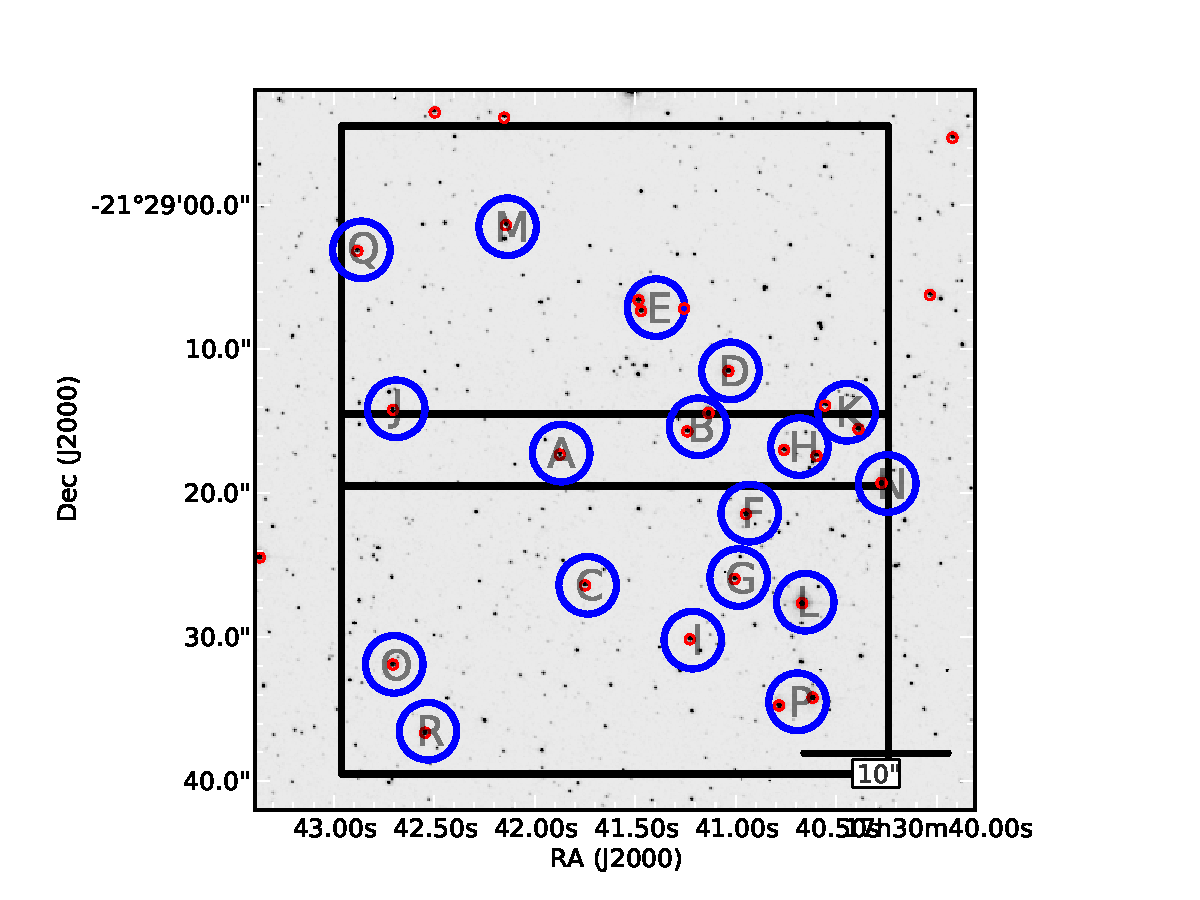
\includegraphics[width=\textwidth]{\plotdir /sn1604_hst_candidates.pdf}
 %  \caption{}
%   \label{fig:sn1604_hst_candidates}
%\end{figure*}

